\chapter{Risoluzione del problema tramite CPLEX}\label{CPLEX} 
\section{Modelli compatti}
I modelli compatti del Travelling Salesman Problem, sono formulazioni matematiche in cui il numero di variabili e di vincoli è polinomiale nella taglia dell'istanza. In particolare, in quelle analizzate in seguito,esse sono entrambe $O(n^2)$, con \textit{n = numero di nodi}.\\
I modelli compatti sono però applicabili solo a grafi orientati. Quindi ciascuna variabile $x_{ij}$ del modello simmetrico deve essere convertita nelle due variabili $x_{ij}$ e $x_{ji}$ del corrispondente modello orientato (vedi Capitolo \ref{intro}). Questo comporta un significativo rallentamento nella computazione della soluzione, in quanto il metodo di risoluzione, nel momento in cui si trovi a scartare un ramo $(i,j)$ dalla possibile soluzione, deve verificare comunque se il corrispondente lato $(j,i)$ potrebbe invece farne parte. Tale controllo risulta però inutile, poichè i due rami vengono associati alla stessa variabile nel modello simmetrico iniziale.
Entrambi i modelli descritti in questa sezione sono stati sviluppati ed il confronto dei tempi di esecuzione delle relative implementazioni viene riportato nella Sezione \ref{compact_perf}.
\subsection{Formulazione di Miller, Tucker e Zemlin}
Nella formulazione del modello di Miller, Tucker e Zemlin, detta anche formulazione sequenziale, per ogni nodo \textit{i} del grafo viene introdotta una nuova variabile $u_i$ , che rappresenta la posizione di tale vertice all'interno del circuito restituito. Vengono introdotti inoltre nuovi vincoli basati sulle variabili $u_i$ che garantiscono la formazione di un unico tour e l'eliminazione di tutti i possibili subtour.\\
Nello specifico il modello utilizzato da Miller, Tucker e Zemlin è il seguente:
\begin{align}
& min \underset{i\in V}\sum{}\underset{j\in V}\sum{c_{ij}\; x_{ij}} \\ \notag \\
& \underset{i\in V}\sum{x_{ih}}\; =\; 1 & \forall\; h\in V \\ \notag \\
& \underset{j\in V}\sum{x_{hj}}\; =\; 1 & \forall\; h\in V \\ \notag \\
& u_i-u_j+n\; x_{ij}\;\leq\; n-1 & \forall\; i,j\in V-\{ 1\} , i\neq j \\ \notag 
\end{align}
\begin{align}
& 0\leq u_i\;\leq\; n-2 & \forall\; i\in V-\{ 1\} \\ \notag 
\end{align}
Esistono però due diversi modi per inserire i vincoli aggiuntivi, legati alle variabili $u_i$,  sfruttando le funzioni di CPLEX.\\
Nel primo questi vengono aggiunti direttamente al modello, durante la costruzione di quest'ultimo. In tal modo, durante la fase di preprocessamento, il programma è già a conoscenza di tutti i vincoli che dovrà rispettare la soluzione ottima e ciò gli permette di apportare ulteriori semplificazioni al modello, rilevandone alcune proprietà utili.\\
Il secondo metodo, invece, prevede l'inserimento nel modello di questi vincoli tramite "lazy constraint". In tal modo i vincoli non sono noti al programma dall'inizio, ma vengono inseriti all'interno di un pool. Nel momento in cui viene calcolata una soluzione, CPLEX ne verificherà la correttezza analizzando l'insieme di vincoli precedentemente definito e se dovesse trovarne uno violato, lo aggiungerà al modello e ripeterà la computazione.
 Questo secondo approccio implementativo permette di eseguire calcoli su un modello di dimensioni inferiori rispetto a quello ottenuto utilizzando il primo metodo. Tuttavia i tempi di calcolo possono aumentare significativamente in quanto CPLEX non può sfruttare la conoscenza dell'intero modello sin dalla sua costruzione. 
Nell'implementazione sviluppata, sono state impiegate entrambe le soluzioni descritte.

\subsection{Formulazione di Gavish e Graves}
Nella formulazione di Gavish e Graves, per impedire la formazione di sub-tour all'interno della soluzione, viene associata a ciascun ramo una nuova variabile $y_{ij}$, che rappresenta il flusso tra i nodi $i$ e $j$. Il modello, legato al problema del commesso viaggiatore, assume la seguente forma:
\begin{align}
& min\underset{i\in V}\sum{\underset{j\in V}\sum{c_{ij}\; x_{ij}}} \\ \notag \\
& \underset{i\in V}\sum{x_{ih}}\;=\;1 & \forall\;h\in V \\ \notag\\
& \underset{j\in V}\sum{x_{hj}}\;=\;1 & \forall\;h\in V \\ \notag\\
& \underset{j\in V}\sum{y_{1j}}\;=\;n-1\\ \notag\\
& \underset{j\in V}\sum{y_{hj}}\;=\;\underset{i\in V}\sum{y_{ih}}\;-1 & \forall\;h\in V-\{1\}\\ \notag\\
& y_{ij}\leq\;(n-1)\;x_{ij} & \forall\;i,j\in V, i\neq j\\ \notag\\
& y_{ii}=0 & \forall\;i\in V\\\notag\\
& y_{i1}=0 & \forall\;i\in V\\\notag
\end{align}
In questo formulazione matematica, i vincoli di subtour elimination vengono sostituiti dai vincoli $(2.9)$, $(2.10)$, $(2.11)$, $(2.12)$, $(2.13)$ che rappresentano rispettivamente: il flusso di uscita dal primo nodo, il bilanciamento dei flussi in ogni singolo nodo, i vincoli di accoppiamento del flusso con un ramo selezionato nella soluzione, il valore del flusso su auto-anelli e il valore del flusso entrante nel primo nodo.\\
La soluzione di questo modello risulta essere però molto lontana dalla convex hull e per migliorarla è possibile sostituire il vincolo $(2.11)$ con: \\
\begin{center}
$y_{ij}\leq\;(n-2)\;x_{ij} \;\;\;\;\;\forall\; i\neq \; j$.\\
\end{center} 
Inoltre per evitare che la soluzione ottima imposti ad $1$ entrambi gli archi orientati $x_{ij}$ e $x_{ji}$, che nell'istanza iniziale sono legati allo stesso arco, viene aggiunto anche il seguente vincolo:
\begin{center}
$x_{ij}+x_{ji}\leq 1\;\;\;\; \forall i,j \in V$ con $i < j$
\end{center}
L'implementazione svolta all'interno del programma utilizza i vincoli $(2.11)$ nella loro prima forma e li inserisce nel modello in fase di costruzione.

\section{Algoritmi Esatti}
\subsection{Loop}
Negli anni '60, Jacques F. Benders sviluppò un approccio generale, applicabile a qualsiasi problema di programmazione lineare, per ridurre il numero esponenziale di vincoli presenti in un modello.\\
Per risolvere tale problema, il metodo Loop costruisce inizialmente il modello senza quei vincoli e li aggiunge solo in seguito durante la risoluzione del problema. L'algoritmo di Benders calcola una soluzione e valuta se questa rispetti tutti i vincoli non inseriti nel modello. Nel caso in cui dovesse trovarne uno che non viene rispettato, lo inserisce nel modello.\\ 
Nel caso del TSP, i vincoli in numero esponenziale sono i Subtour Elimination (SEC), che hanno la seguente forma:
\begin{align}
&\underset{e\in E(S)}\sum{x_{e}} \leq \mid S\mid - 1\;\forall\;S\underset{\neq}{\subset}V\; : \; \mid S\mid\geq 2
\end{align}
o equivalentemente:
\begin{align}
&\underset{e\in \delta(S)}\sum{x_{e}}\geq 2\;\forall\;S\underset{\neq}{\subset}V\; : \; \mid S\mid\geq 2
\end{align}
Definendo il modello per il problema del commesso viaggiatore, vengono rimossi i SEC. In seguito viene risolto il problema e nel caso in cui la soluzione abbia più di una componente connessa, viene aggiunto al modello un vincolo di Subtour Elimination per ogni ciclo generato. Il processo viene ripetuto iterativamente, come mostrato nel seguente pseudocodice, fino a che la soluzione non sia costituita da un unico tour.\\\\
\begin{algorithm}[H]
\DontPrintSemicolon
\KwIn {$\mathtt{model}$= Modello TSP simmetrico senza vincoli di Subtour Elimination\newline}
\KwOut {$\mathtt{x}$= soluzione intera senza subtour}
\BlankLine 
 $\mathtt{x} \gets$ solve(model)\;
 $\mathtt{ncomps} \gets$ comps(x)\;
 \BlankLine 
 \While{$\mathtt{ncomps} \geq 2$}{
  Aggiungi $\underset{e\in \delta(S_k)}\sum{x_{e}}\leq \mid S_k\mid - 1\;\forall$ componente connessa $S_k$\;
  \BlankLine  
  \If{$\mathtt{ncomps} \geq 2$}{
    \BlankLine
    $\mathtt{x} \gets$ solve(model)\;
    $\mathtt{ncomps} \gets$ comps(x)\;
  }
 }
 \caption{LOOP}
\end{algorithm}
\vspace{0.5 cm}
All'aumentare del numero di vincoli inseriti nel modello, il costo della soluzione peggiora o resta invariato rispetto al costo di quella elaborata all'iterazione precedente del metodo Loop.\\
Il numero di iterazioni che vengono effettuate dall'algoritmo non è calcolabile a priori e potrebbe essere anche molto elevato. Nel caso peggiore verranno inseriti tutti i vincoli di Subtour Elimination, ovvero un numero esponenziale di disequazioni, soprattutto nel caso di istanze clusterizzate.\\
L'introduzione di nuovi SEC, solo nel momento in cui si presenta una loro violazione, permette di ridurre la dimensione del modello ma diminuisce l'attività di pre-processamento svolta da CPLEX prima di risolvere il problema. Inoltre il problema principale del metodo Loop è la generazione di un nuovo albero completo di branching ad ogni nuova iterazione.\\
In passato, con le versioni del MIP solver di CPLEX, questa operazione era molto onerosa mentre attualmente il metodo loop garantisce la risoluzione, anche di istanze molto grandi, in tempi ragionevoli. Questo non accade invece per il Branch \& Bound in quanto vengono aggiunte nuove ramificazioni all'albero già esistente.\\
Il metodo Loop può essere modificato svolgendo prima l'algoritmo Loop con l'aggiunta di parametri differenti da quelli utilizzati di default del risolutore CPLEX e solo in seguito effettuando l'algoritmo di Benders, questa volta utilizzando le impostazioni di default di CPLEX. \\
Quest'ottimizzazione è basata sul fatto che CPLEX salvi alcune soluzioni, ottenute in precedenza dal risolutore sullo stesso modello, e le sfrutti come bound nel nuovo modello. Per questo motivo, la soluzione metaeuristica ottenuta nella prima fase viene sfruttata come bound nella seconda.

\subsection{Branch \& Cut}
Come precedentemente anticipato, CPLEX effettua inizialmente una fase di pre-processamento in cui semplifica il modello, e terminata questa operazione inizia ad eseguire la fase di Branch \& Cut. Ogni volta che calcola una nuova soluzione $x^*$, prima di dichiarare se è l'ottimo o di scartarla e proseguire a sviluppare i successivi rami dell'albero decisionale, applica dei tagli e degli algoritmi euristici per aggiornarla (vedi Figura \ref{Albero_decisionale}).\\
\begin{figure}[h] 
\begin{center} 
  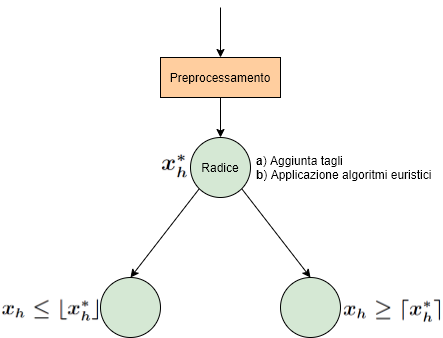
\includegraphics[scale=0.6]{Images/albero_decisionale}\\ 
  \caption{\footnotesize{Albero decisionale del Branch and Cut}}
  \label{Albero_decisionale} 
\end{center} 
\end{figure}
Nello sviluppo del Branch \& Cut, per ciascun nodo dell'albero decisionale, vengono considerati due bound:
\begin{itemize}
\item{\textbf{Upper Bound}\\
viene definito dagli algoritmi euristici utilizzati.
}
\item{\textbf{Lower Bound}\\
viene definito dal rilassamento del problema e dall'azione di diversi tagli.
}
\end{itemize}
CPLEX permette di personalizzare i tagli da applicare nel Branch \& Cut e di inserire iterativamente i Subtour Elimination relativi alle componenti connesse nella soluzione a cui verrà applicato il taglio. Per fare ciò l'utente può implementare questi vincoli mediante delle callback, \textit{lazy constraints callback}, utilizzate per aggiungere lazy constraints al modello.\\
Le lazy callback implementate vengono chiamate solo nel momento in cui deve essere aggiornato l'incumbent e se necessario CPLEX aggiungerà al modello i vincoli violati. Verranno quindi invocate più frequentemente all'inizio del calcolo della soluzione del problema, e meno nelle iterazioni successive. Questo poichè essendoci in partenza meno vincoli, sarà più facile per la soluzione soddisfarli tutti.\\
A differenza dei \textit{lazy constraint}, con l'utilizzo delle \textit{lazy callback} i vincoli non sono costantemente presenti in un pool, ma vengono generati "al volo" al momento necessario.  Quest'operazione velocizza notevolmente il calcolo della soluzione ottima, in quanto permette a CPLEX di non dover calcolare nuovamente l'albero decisionale dalla radice, ma di procedere nel suo sviluppo aggiungendo nuovi rami.\\
In particolari casi, però, CPLEX può ritenere più conveniente distruggere l'intero albero decisionale finora calcolato e ricominciare la computazione dalla radice. Questo può avvenire in qualunque punto dell'elaborazione della soluzione ottima e utilizzando istanze abbastanza grandi, diventa evidente visionando i log di CPLEX.\\
Attraverso l'utilizzo delle callback è possibile accedere a numerose informazioni relative alle elaborazioni fatte da CPLEX. Per questo motivo, alcune procedure vengono automaticamente disattivate, affinché l'utente non possa venire a conoscenza di particolari dettagli implementativi. Un esempio è la dynamic search. Tale avvenimento può causare un rallentamento nel calcolo della risoluzione.\\
Nelle ultime versioni di CPLEX sono state  introdotte le \textit{generic callback} che permettono di mantenere attivi tutti i meccanismi presenti all'interno del programma per la computazione della soluzione e di ovviare quindi a questo problema.  
\subsection{Patching algorithm}
Negli algoritmi analizzati nelle precedenti sottosezioni può succedere che CPLEX, prima di trovare il tour ottimo, computi soluzioni con più componenti connesse. Per evitare che vengano scartate senza essere sfruttate è possibile utilizzare questo semplice algoritmo euristico, il quale si pone l'obiettivo di convertirle in un tour ammissibile.\\
Date due componenti connesse all'interno della soluzione calcolata, queste vengono unite in una sola grazie all'eliminazione di un ramo ciascuna $\{a, a'\}$ e  $\{b, b'\}$ e alla selezione di altri due rami che fungano da collegamento tra i quattro vertici selezionati ($\{a, b\}$ e $\{a', b'\}$ o $\{a, b'\}$ e $\{a', b\}$) (vedi Figura \ref{patching}).\\
\begin{figure}[h] 
\begin{center} 
  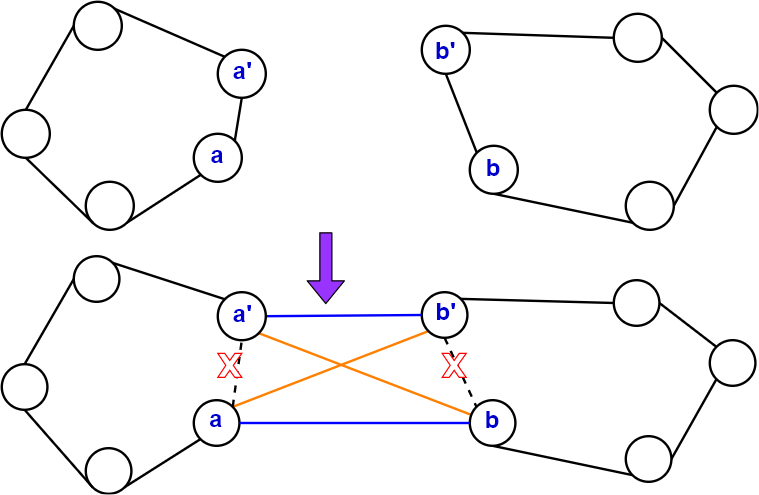
\includegraphics[scale=0.38]{Images/patching}
  \caption{\footnotesize{Esempio di patching}} \label{patching} 
\end{center} 
\end{figure}
Per scegliere quale ramo per ogni componente connessa sia più conveniente eliminare e con quale sia più conveniente sostituirlo, è necessario minimizzare la variazione del costo complessivo della soluzione che quest'operazione comporterebbe, cioè scegliere il minimo tra: \\\\
$min \begin{cases}
\Delta \;(a,b)\;=c_{ab'} + c_{ba'} - c_{aa'} - c_{bb'}\\ 
\Delta' \;(a,b)\;=c_{ab} + c_{b'a'} - c_{aa'} - c_{bb'}\\ 
\end{cases}
\forall \; a,b \in V : comp(a)\neq comp(b)$
\\\\
L'operazione di fusione di due componenti connesse dev'essere essere ripetuta finché la soluzione non diventa ammissibile. In questo modo, al termine, è possibile restituire una soluzione accettabile, ma senza garanzia che sia ottima.\\
Nella nostra implementazione è stato scelto di mantenere invariata ad ogni iterazione una delle componenti connesse e di espanderla fondendola a quella più vicina. Grazie a questa scelta viene minimizzato il numero di rami per cui è necessario modificare la struttura dati che li memorizza.\\
Per poter implementare l'algoritmo è necessario utilizzare due diversi tipi di callback messe a disposizione da CPLEX. La prima appartiene alla tipologia delle \textit{lazy constraint callback}  ed è necessaria per ricevere la soluzione trovata dal programma e rielaborarla. A questa soluzione viene applicato l'algoritmo di patching ed il risultato viene memorizzato all'interno in una struttura dati accessibile anche dalla seconda callback dell'utente. Per garantire che le user-callback siano thread-safe, la struttura dati nominata è stata organizzata di  modo tale che ogni thread acceda ad una sua specifica porzione.\\
La seconda callback necessaria è un \textit{heuristic callback} e permette all'utente di suggerire a CPLEX una soluzione da cui proseguire la computazione. Questa soluzione sarà quella memorizzata nella struttura dati dalla prima callback e verrà utilizzata dal programma solo nel caso in cui sia migliore dell'incumbent attuale.\\
Utilizzando, invece, le \textit{generic callback} non è necessario implementare due diverse user-callback. E' sufficiente invocare la callback in due differenti contesti: uno per ricevere la soluzione di CPLEX, CPX\_CALLBACKCONTEXT\_CANDIDATE, e l'altro per suggerire il risultato del patching ,CPX\_CALLBACKCONTEXT\_LOCAL\_PROGRESS. I due casi andranno poi gestiti dall'interno della funzione stessa.\\
Complessivamente il costo di quest'algoritmo è $O(n^2)$, dove $n$ è il numero di nodi. %verificare

\begin{algorithm}[h]
\DontPrintSemicolon
\KwIn {$\mathtt{x}$= soluzione di un problema di TSP con più componenti connesse\newline}
\KwOut {$\mathtt{y}$= soluzione intera formata da un'unica componente connessa}
\BlankLine
$\mathtt{n\_comps \gets} numero componenti connesse della soluzione$\;
\BlankLine
$\mathtt{c_1\gets}\{0,...,0\}$\;
\BlankLine
\While{$n\_comps > 1$}{
\BlankLine
$\mathtt{c_1 \gets first\_subtour(}x\mathtt{)}$\;
\BlankLine
$\mathtt{c_2 \gets nearest\_subtour(}c_1\mathtt{)}$\;
\BlankLine
$\mathtt{merge\_component(}c_1,c_2\mathtt{)}$\;
\BlankLine
$\mathtt{update(}n\_comps\mathtt{)}$\;
}
$\mathtt{y \gets} c_1$\;
\caption{Patching}
\end{algorithm}

\section{Algoritmi Math-Euristici}
Gli algoritmi euristici sono progettati per risolvere istanze del problema in tempi significativamente più brevi rispetto agli algoritmi esatti. Di conseguenza, però, al termine della computazione non garantiscono di ottenere una soluzione ottima, ma solo una sua buona approssimazione ammissibile. Gli algoritmi Math-euristici sfruttano l'approccio utilizzato dai metodi euristici unito alla programmazione matematica, introducendo nuovi vincoli al modello. L'algoritmo che maggiormente rappresenta questo metodo è il Soft Fixing (vedi Sezione \ref{soft fixing}). \\
Durante la computazione della soluzione CPLEX utilizza diversi algoritmi euristici e math-euristici e variando alcuni parametri è possibile variare la frequenza con cui vengono applicati o il tempo a loro dedicato. 

\subsection{Hard Fixing}\label{hard fixing}
Un primo algoritmo math-euristico di semplice implementazione è l'Hard Fixing, composto dalle seguenti fasi:
\begin{enumerate}
\item{Impostazione di un time limit per la computazione di una soluzione;}
\item{Calcolo della soluzione;}
\item{Selezione, in maniera randomica, di un sottoinsieme di rami appartenenti alla soluzione ottima (Figura \ref{selezione_rami}). 
Il numero di questi è definito da una percentuale fissata sul totale dei lati scelti. Le variabili dei rami selezionati, sono impostate al valore $1$.}
\end{enumerate}
\begin{figure}[h] 
\begin{center} 
  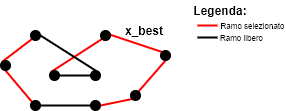
\includegraphics[scale=0.38]{Images/x_best} 
  \caption{\footnotesize{Selezione rami}}
  \label{selezione_rami} 
\end{center} 
\end{figure}
Questi passaggi vengono eseguiti in maniera ciclica per un numero fissato di iterazioni. In questo modo, ad ogni computazione della soluzione, CPLEX dovrà risolvere un problema più semplice di quello originale, essendo molte variabile del modello già selezionate nella \textbf{Fase 3} dell'iterazione precedente.\\
All'interno del programma sviluppato, il time limit nominato nella \textbf{Fase 1} è dato da una frazione della deadline complessiva inserita dall'utente e dipende dal numero di diverse percentuali che si desidera utilizzare. All'ultima iterazione il time limit viene ricalcolato in base al tempo rimanente a disposizione, rispetto alla deadline complessiva inserita dall'utente. Ad ogni computazione il costo della soluzione potrà solo migliorare o restare invariato rispetto alla precedente soluzione calcolata.\\
La percentuale relativa al numero di rami da fissare può variare ad ogni iterazione. Generalmente viene utilizzata una percentuale alta nelle prime iterazioni, in cui la soluzione non è ancora stata raffinata, e viene ridotta nelle successive, in modo da aumentare i gradi di libertà per CPLEX nella computazione della soluzione.\\
La selezione in maniera randomica degli archi nella \textbf{Fase 3}, garantisce che l'algoritmo termini poichè non vengano fissate sempre le stesse variabili. 
% LEGGILA
Particolare attenzione deve essere posta al fatto di lasciare nell'insieme dei rami scelti randomicamente solo quelli selezionate all'iterazione immediatamente precedente. Nell'implementazione sviluppata, le percentuali utilizzate sono state memorizzate in un vettore in questo ordine $\lbrace$ 90, 75, 50, 25, 10, 0 $\rbrace$.
Di seguito viene inoltre riportato lo pseudocodice dell'implementazione sviluppata:\\
\begin{algorithm}[h]
\DontPrintSemicolon
\KwIn {$\mathtt{model}$= modello TSP simmetrico senza vincoli di Subtour Elimination \newline
$\mathtt{deadline}$= time limit complessivo dell'algoritmo\newline
$\mathtt{percentage}$= array con i valori delle percentuali di fissagio degli archi\newline
$\mathtt{num\_nodi}$= numero di nodi dell'istanza TSP\newline}
\KwOut {$\mathtt{x}$= soluzione intera senza subtour}
\BlankLine
$\mathtt{n \gets}0$\;
\BlankLine
\While{$expired\_time < deadline$}{
 \BlankLine\BlankLine
 $\mathtt{setTimeLimit()}$\;
 $\mathtt{x \gets solve(}model\mathtt{)}$\;
 \BlankLine\BlankLine
 \For{$\mathtt{j \gets}0$ \KwTo $num\_nodi-1$}{
   $k \gets random(0,1)$\;
   \BlankLine\BlankLine
   \If{$  100*k \leq percentage[n\;mod\;lenght(percentage)]  $}{
     \BlankLine
     $Aggiungi \;\;\mathtt{x\_best[j]}\;\;to\;\;S\;where\;S=\{edges\;to\;fix\}$
   }
   \BlankLine
}
\BlankLine
\ForAll{$x_{ij} \in S$}{
$\mathtt{x_{ij} \gets}1$\;
\BlankLine
}
\BlankLine
$\mathtt{n \gets}n+1$\;
\BlankLine
}
\caption{Hard Fixing}
\end{algorithm}

\subsection{Soft Fixing}\label{soft fixing} %controlla che siano local branching
Il metodo seguente fa utilizzo di vincoli aggiuntivi, detti di \textbf{Local Branching}. L'approccio utilizzato è simile a quello dell'Hard Fixing, in questo caso però la scelta delle variabili da imporre a $1$ non avviene in maniera randomica ma viene lasciata a CPLEX.\\
Partendo da una soluzione intera ammissibile del TSP $x^H$, viene aggiunto un vincolo sulle variabili con valore $1$ in $x^H$:\\
$$\underset{e\in E\; : \; {x_e}^{H}=1}\sum{x_e}\;\geq\; 0.9\;n$$
dove la sommatoria indica il numero di variabili, uguali a $1$ in $x^H$, che non cambieranno il loro valore e \textbf{n} indica il numero di archi selezionati dalla soluzione, pari al numero di nodi.\\
In questo caso, il vincolo permetterà a CPLEX di fissare il 90\% dei rami scelti in $x^H$ e avere il 10\% di libertà.
Un modo alternativo di scrivere lo stesso vincolo è il seguente:
$$\underset{e\in E\; : \; {x_e}^{H}=1}\sum{x_e}\;\geq\; n-k$$
dove $k\;=\;2,...,20$ e rappresenta i gradi di libertà di CPLEX nel calcolare la nuova soluzione.\\
Ad ogni iterazione dell'algoritmo viene aggiunto un nuovo vincolo di \textit{Local Branching}, basato sull'attuale soluzione restituita da CPLEX, e viene rimosso il vincolo inserito nel modello all'iterazione precedente.\\
Non scegliendo in maniera randomica i lati da selezionare, come invece accade nell'Hard Fixing, se non dovesse esserci alcun miglioramento del costo e quindi cambiamento della soluzione, i lati selezionati da CPLEX con il nuovo vincolo sarebbero gli stessi dell'iterazione precedente. Per ovviare tale problema, il valore di k viene inizializzato a 2 e, nel caso in cui non dovesse migliorare la soluzione, viene incrementato.\\
Da dati sperimentali, si è appurato come questo metodo aiuti CPLEX a convergere più velocemente alla soluzione ottima e che valori di k superiori a 20 non aiutino a raggiungere risultati migliori.\\
Normalmente per poter analizzare lo spazio delle soluzioni è necessario enumerare tutti gli elementi al suo interno. Grazie all'aggiunta di un vincolo di \textit{Local Branching} è, invece, possibile eseguire quest'operazione in maniera più semplice e veloce.\\ 
%permette di analizzare in maniera più semplice e veloce lo spazio delle soluzioni. Normalmente per farlo, dovrebbero essere enumerati gli elementi di questo spazio, ma ciò comporterebbe la creazione di un numero molto elevato di possibili soluzioni per via della NP-difficoltà del TSP.\\
Definita una soluzione intera ammissibile $x^H$ e utilizzando la distanza di Hamming, le soluzioni $k-opt$, rispetto ad $x^H$, sono quelle che hanno distanza k da essa (vedi Figura \ref{opt}).\\
\begin{figure}[h] 
\begin{center} 
  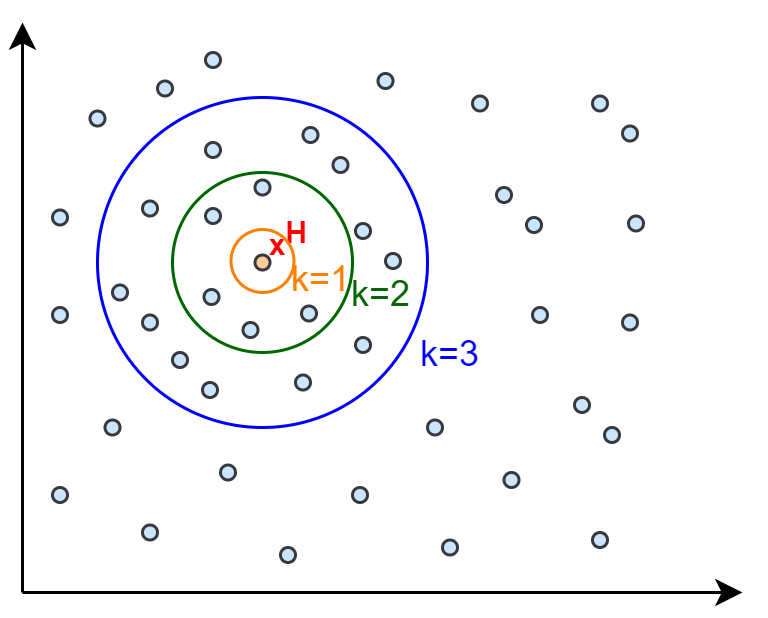
\includegraphics[scale=0.38]{Images/opt}
  \caption{\footnotesize{Spazio delle soluzioni e distanza di Hamming.}} \label{opt} 
\end{center} 
\end{figure}
%Se, invece del \textit{Local Branching}, venisse utilizzata l'enumerazione delle soluzioni, 
Utilizzando l'enumerazione delle soluzione dovrebbero essere generate, per \textbf{k} generico, circa $n^k$ soluzioni a distanza k da $x^H$. In seguito dovrebbero essere analizzate tutte per individuare quella con costo minore di $x^H$.\\
L'utilizzo del \textit{Local Branching} può essere adottato con anche problemi generici e non solo con TSP. Di seguito viene riportato l'approccio da seguire per generare tutte le soluzioni a distanza minore o uguale di R dalla soluzione euristica di partenza $x_H$:
\begin{align}
& min \{ c^T x:\;\;Ax=b,\;x\in\{0,1\}^n\} \\ \notag \\
& \underset{j\in E:{x_j}^H=0}\sum{x_j}\;+ \underset{j\in E:{x_j}^H=1}\sum{1-x_j}=\; \leq R
\end{align}
dove $(2.17)$ rappresenta la distanza di Hamming della nuova soluzione computata $x$ da $x_H$. L'obiettivo del Soft Fixing è cercare di migliorare il costo della soluzione, guardando quelle più vicine possibili a quella attuale. Nella Figura \ref{local_exe} viene riportato un esempio di una possibile evoluzione dell'algoritmo nella ricerca dell'ottimo, evidenziandone le soluzioni trovate di volta in volta.
\begin{figure}[H] 
\begin{center} 
  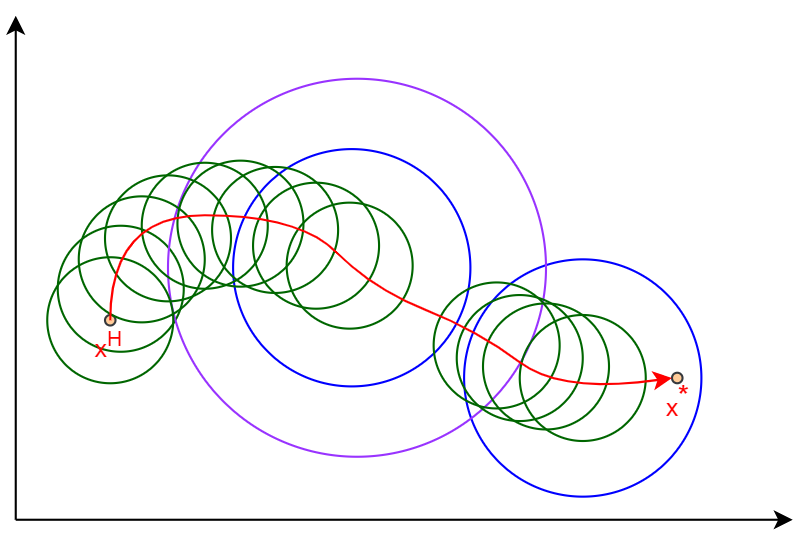
\includegraphics[scale=0.38]{Images/local_exe}
  \caption{\footnotesize{Esempio di esecuzione dell'algoritmo nello spazio delle soluzioni.}} \label{local_exe} 
\end{center} 
\end{figure}